\section{Evaluating Performance}
\label{sec:results}

In this section, we test the \emph{Prediction Algorithm} presented in Section~\ref{subsec:prediction_algorithm} with the data present on the graph.

\subsection{Data Partitioning}

\subsubsection{Train Test Split}
\label{subsec:train_test_split}

As with many other classification problems, the \emph{Bayesian Algorithm} is prone to overfitting~\cite{mitchellml1997}. In this particular case, since the information presented in Section~\ref{subsec:income_homophily} shows that users tend to communicated with users of the same socioeconomic level, by running the algorithm in the complete data and using the same users as part of the features and of the labels, we would erroneously be having more data per user than we would have when modelling the problem.

An easy way to avoid this problem is by doing a simple \emph{Train Test Split}, where the data in $B$ is separated into two disjoint groups, $B = B_{\train} \cup B_{\test}$ and $B_{\train} \cap B_{\test} = \varnothing$, where $\left| B_{\train} \right| = \sfrac{4}{5} \cdot \left| B \right|$ and $\left| B_{\test} \right| = \sfrac{1}{5} \cdot \left| B \right|$.

\subsubsection{Erasing Uninformative Data}

Given that $\left| B \right| \ll \left| V \right|$ and that $G$ is sparse, the vast majority of users don't have any kind of contact with users of the bank. For this reason it's useless to evaluate the performance of the algorithm using all the nodes, and therefore the \emph{Testing Set} used in this thesis will instead focus on the bank users that have at least one contact with another bank user. This approach is formalized in Equation~\ref{eq:inner_graph}.

\begin{equation}
\label{eq:inner_graph}
\begin{gathered}
\hat{E} = \left\{ e \in E \mid e_o \in B_{\train} \lor e_d \in B_{\train} \right\} \\
\hat{B}_{\test} = B_{\test} \cap \left( \hat{E}_o \cup \hat{E}_d \right)
\end{gathered}
\end{equation}

This approach works perfectly when $\varpi = \contacts$. However, it's possible that for other values of $\varpi$ there won't be any information available in $\hat{B}_{\test}$ in the case of users who either didn't receive any call from a bank user or didn't receive any message.

The equations~\ref{eq:inner_graph_call} and~\ref{eq:inner_graph_sms} formalize new variables to use for informative data in those cases.

\begin{equation}
\label{eq:inner_graph_call}
\begin{gathered}
\hat{E}^{\calls} = \left\{ e \in E \mid e_c > 0 \land \left( e_o \in B_{\train} \lor e_d \in B_{\train} \right) \right\} \\
\hat{B}^{\calls}_{\test} = B_{\test} \cap \left( \hat{E}^{\calls}_o \cup \hat{E}^{\calls}_d \right) \\
\end{gathered}
\end{equation}

\begin{equation}
\label{eq:inner_graph_sms}
\begin{gathered}
\hat{E}^{\sms} = \left\{ e \in E \mid e_s > 0 \land \left( e_o \in B_{\train} \lor e_d \in B_{\train} \right) \right\} \\
\hat{B}^{\sms}_{\test} = B_{\test} \cap \left( \hat{E}^{\sms}_o \cup \hat{E}^{\sms}_d \right)
\end{gathered}
\end{equation}

\subsubsection{Rebalancing Labels}

Since the testing data $B_{\test}$ was a random subsample of a balanced set (see Section~\ref{subsec:train_test_split} and Section~\ref{subsec:discrimination_by_wealth}), it was also balanced itself\maybe{Make sure $B$ refers only to bank users \textbf{in the telco}}. However, since \emph{High Income} users tend to communicate more often than \emph{Low Income} ones, $\hat{B}_{\test}$ is unbalanced and has a significant bias for high-income users.

Since the income categories tend to be balanced in the real world, this isn't wanted. However, since it's not necessary to use the entire \emph{Testing Set} for testing the algorithm, a simple way would be to create a new, balanced, and final testing set, $\Upsilon \subseteq \hat{B}_{\test}$ containing all users from $\hat{B}_{\test}$ \emph{Low Income}, along with a random sample of the same size with \emph{High Income}.

\begin{equation}
\label{eq:upsilon}
\begin{gathered}
\begin{aligned}
\Upsilon^{\low} &= \hat{B}_{\test} \cap H_1 \\
\Upsilon^{\high} &\subseteq \hat{B}_{\test} \cap H_2
\end{aligned} \\
\left| \Upsilon^{\low} \right| = \left| \Upsilon^{\high} \right| \\
\Upsilon = \Upsilon^{\low} \cup \Upsilon^{\high}
\end{gathered}
\end{equation}

$\Upsilon$ will be the only \emph{Testing Set} used from now on, while $B_{\train}$ will be used as training set.

Additionally, the sets $\Upsilon^{\calls}$ and $\Upsilon^{\sms}$ refer to similar sets which are taken from users from the \emph{Testing Set} that had at least one call or sent at least one SMS, respectively, to another user in the \emph{Training Set}.

\subsubsection{Set Magnitudes}

While the new set $\Upsilon$ contains significantly less users than the original set $B$, it still has a sufficient amount of people to make a prediction. Table~\ref{tab:partition_numbers} shows the number of users that remain after every trim used in this Subsection.

\begin{table}
\centering
\begin{tabular}{l r r r}
\toprule
Set & Total Size & High Income & Low Income \\
\midrule
$B$ & \num{5402959} & \num{2702628} & \num{2700331} \\
$B_{\test}$ & \num{1080592} & \num{540526} & \num{540066} \\
$\hat{B}_{\test}$ & \num{53691} & \num{35215} & \num{18476} \\
$\Upsilon$ & \num{36952} & \num{18476} & \num{18476} \\
$\Upsilon^{\calls}$ & \num{30715} & \num{15653} & \num{15062} \\
$\Upsilon^{\sms}$ & \num{11909} & \num{6046} & \num{5863} \\
\bottomrule
\end{tabular}
\caption{Amount of users in the \emph{Testing Set} after trimming it several times to prevent overfitting while keeping the labels balanced}
\label{tab:partition_numbers}
\end{table}

\subsection{Algorithm Performance}

The \emph{Bayesian Algorithm} will be ran for every $\varpi \in \left\{ \contacts, \calls, \etime, \sms \right\}$. For every possible configuration, we present 3 plots for $\Theta = 0.005$.

\begin{itemize}
	\item A \textbf{histogram} presenting the distribution of the $p_v$ values which result from applying Equation~\ref{eq:beta_theta_ppf} presented in Section~\ref{subsec:modelling_users} to each distinct \emph{Beta Distribution}.
	\item An \textbf{Receiver Operating Characteristic Curve}, showing the tradeoff of \emph{False Positive Rate} to \emph{True Positive Rate} when selecting every possible $\tau$. The \emph{Area Under the Curve} is marked, as this is the metric that is being maximized when selecting the correct $\varpi$.
	\item An \textbf{Accuracy Curve}, which shows the \emph{Accuracy} of the predictor by its \emph{False Positive Rate}. $\tau$ is chosen as to maximize this value.
\end{itemize}

\subsubsection{Inferring by Calls}

\begin{figure}[h]
\centering
\begin{subfigure}[t]{\textwidth}
	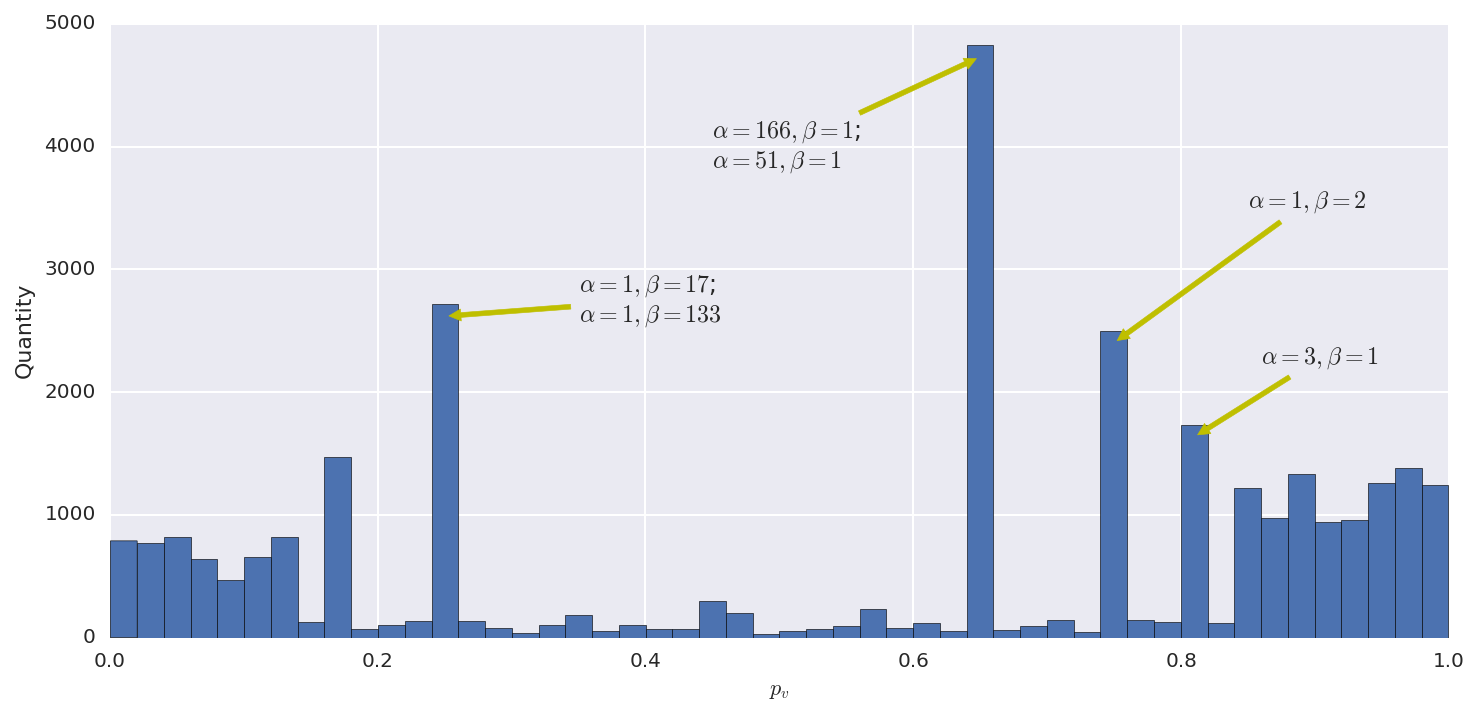
\includegraphics[width=\textwidth]{figures/bayes/hist_calls.png}
\end{subfigure}

\begin{subfigure}[b]{.49\textwidth}
	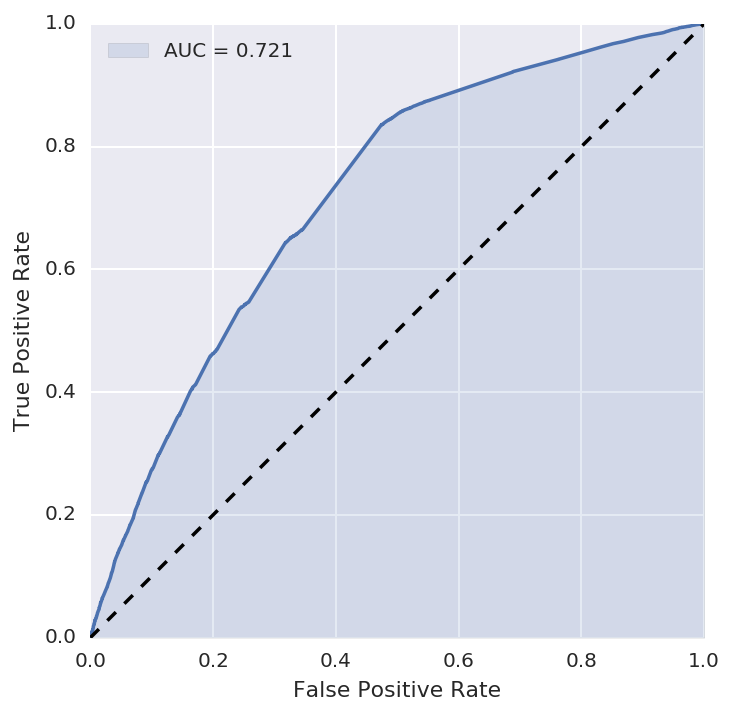
\includegraphics[width=\textwidth]{figures/bayes/roc_calls.png}
\end{subfigure}
\begin{subfigure}[b]{.49\textwidth}
	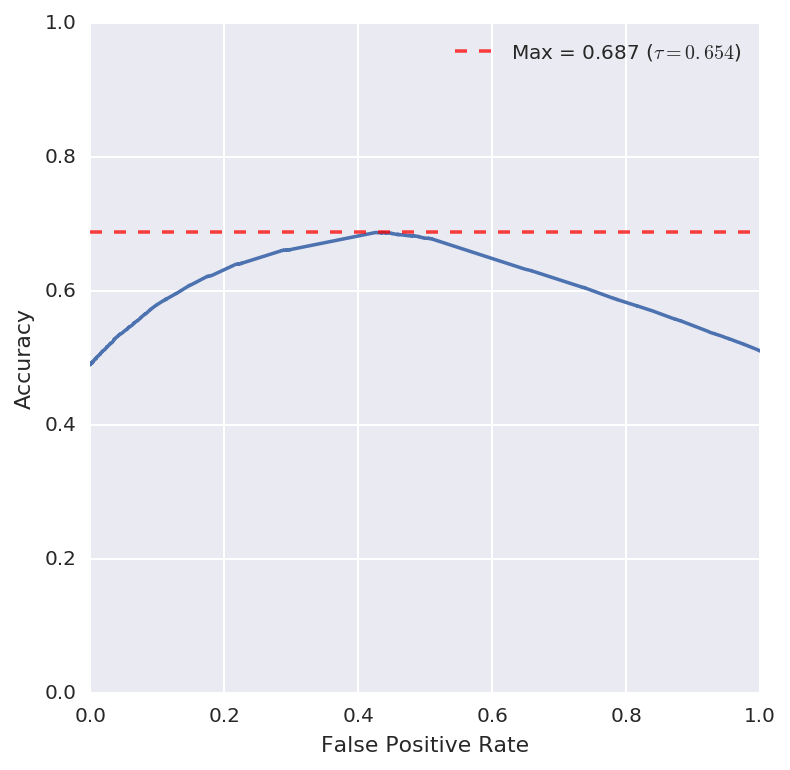
\includegraphics[width=\textwidth]{figures/bayes/accuracy_calls.png}
\end{subfigure}
\caption{Graphics representing the performance of the data when $\varpi = \calls$, using \emph{Beta Distributions} from the data in $\Upsilon^{\calls}$}
\end{figure}

\subsubsection{Inferring by Time}

\begin{figure}[h]
\centering
\begin{subfigure}[t]{\textwidth}
	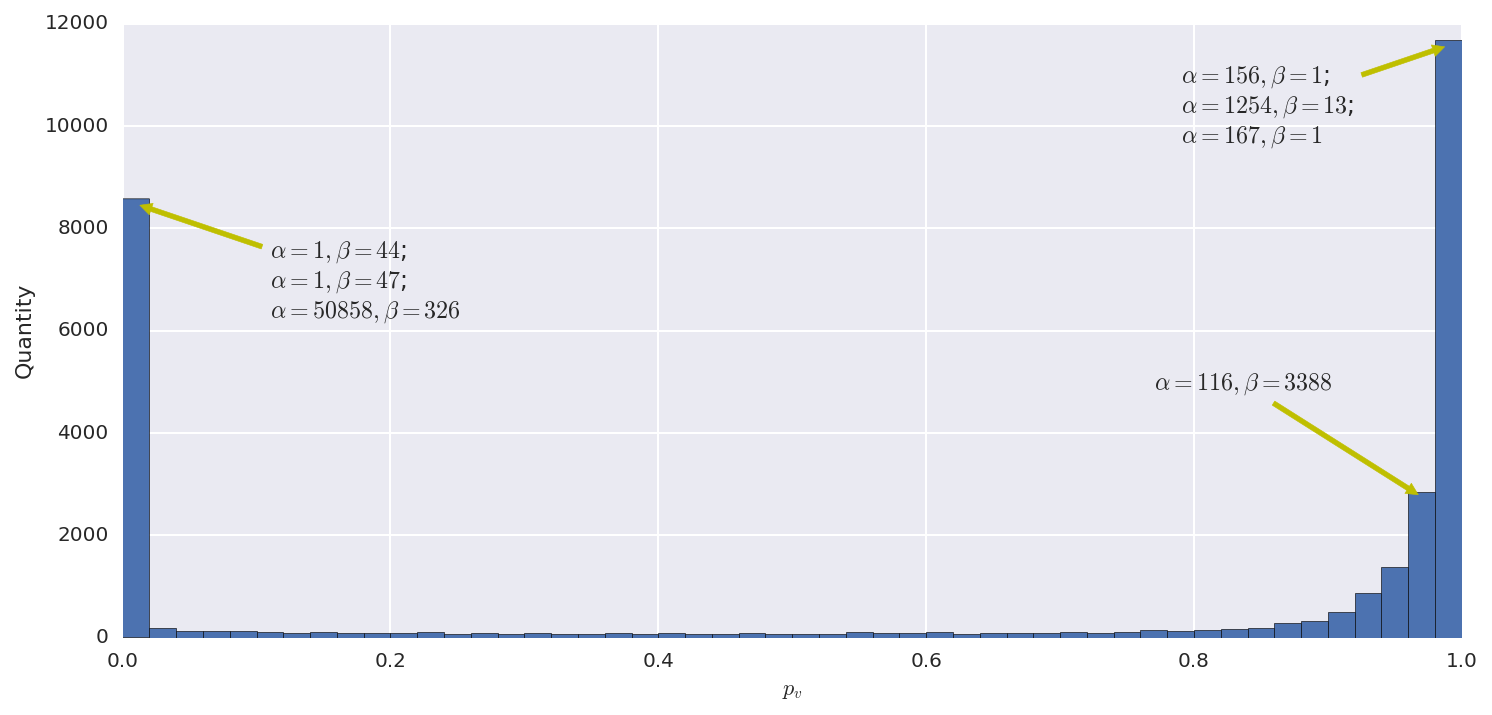
\includegraphics[width=\textwidth]{figures/bayes/hist_time.png}
\end{subfigure}

\begin{subfigure}[b]{.49\textwidth}
	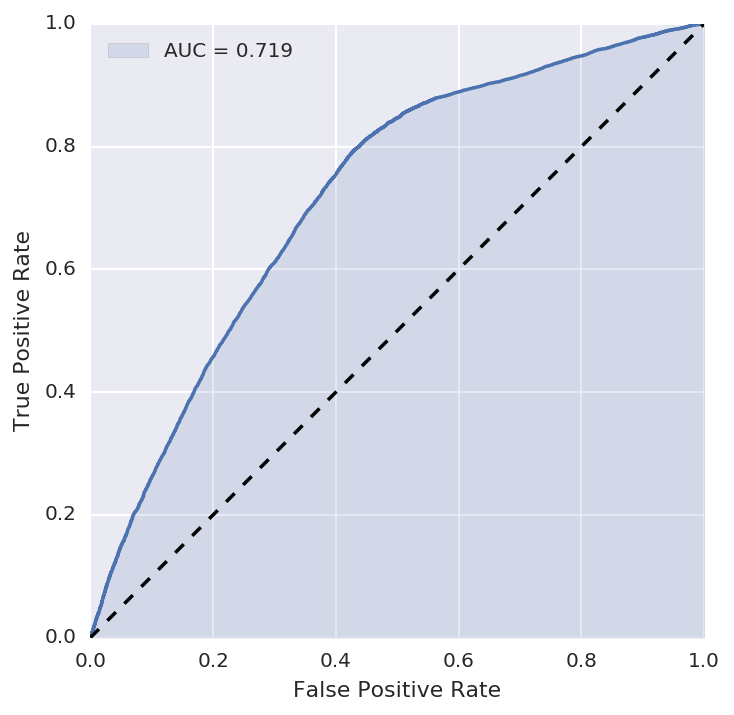
\includegraphics[width=\textwidth]{figures/bayes/roc_time.png}
\end{subfigure}
\begin{subfigure}[b]{.49\textwidth}
	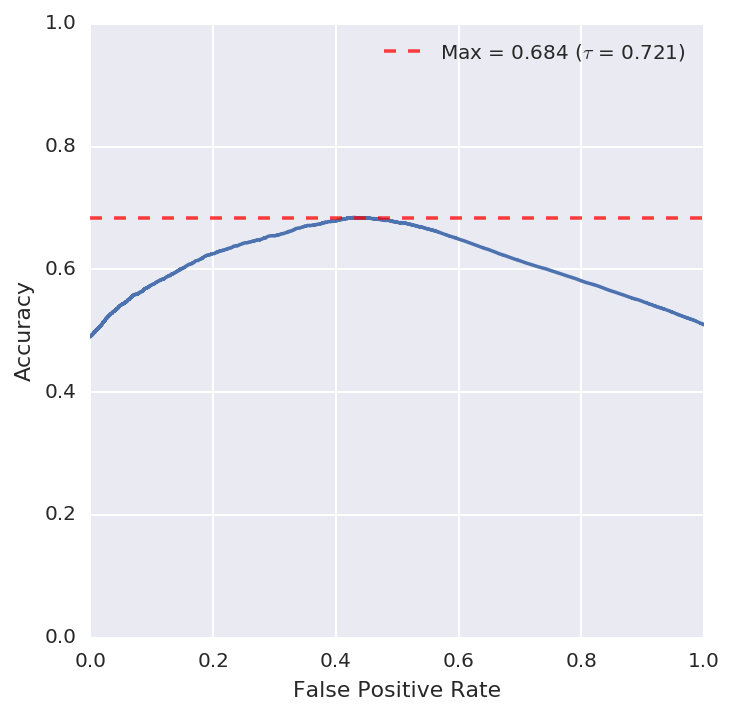
\includegraphics[width=\textwidth]{figures/bayes/accuracy_time.png}
\end{subfigure}
\caption{Graphics representing the performance of the data when $\varpi = \etime$, using \emph{Beta Distributions} from the data in $\Upsilon^{\calls}$}
\end{figure}

\subsubsection{Inferring by SMS}

\begin{figure}[h]
\centering
\begin{subfigure}[t]{\textwidth}
	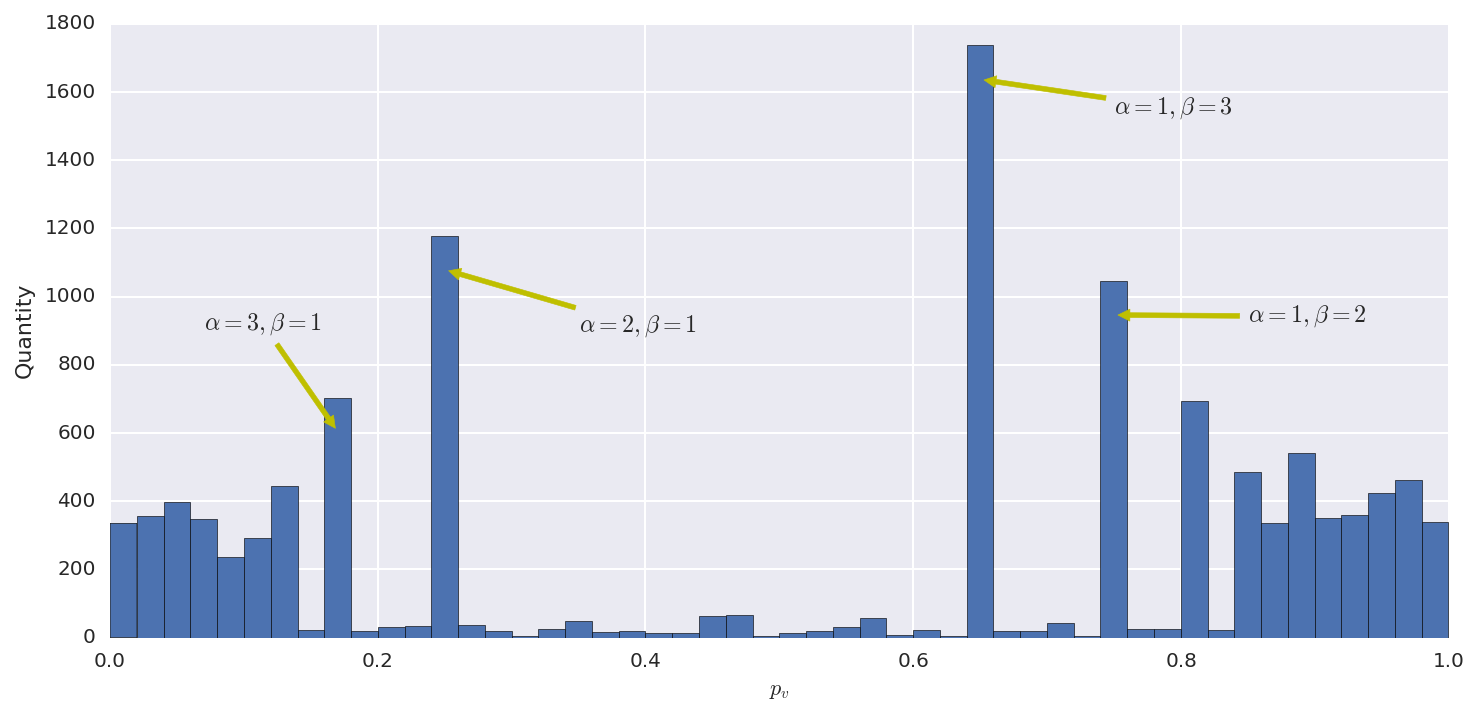
\includegraphics[width=\textwidth]{figures/bayes/hist_sms.png}
\end{subfigure}

\begin{subfigure}[b]{.49\textwidth}
	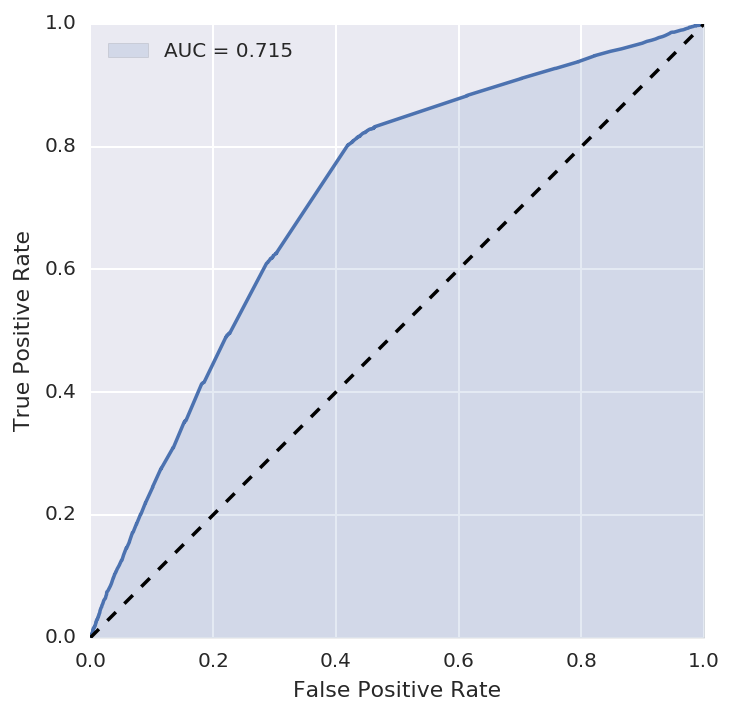
\includegraphics[width=\textwidth]{figures/bayes/roc_sms.png}
\end{subfigure}
\begin{subfigure}[b]{.49\textwidth}
	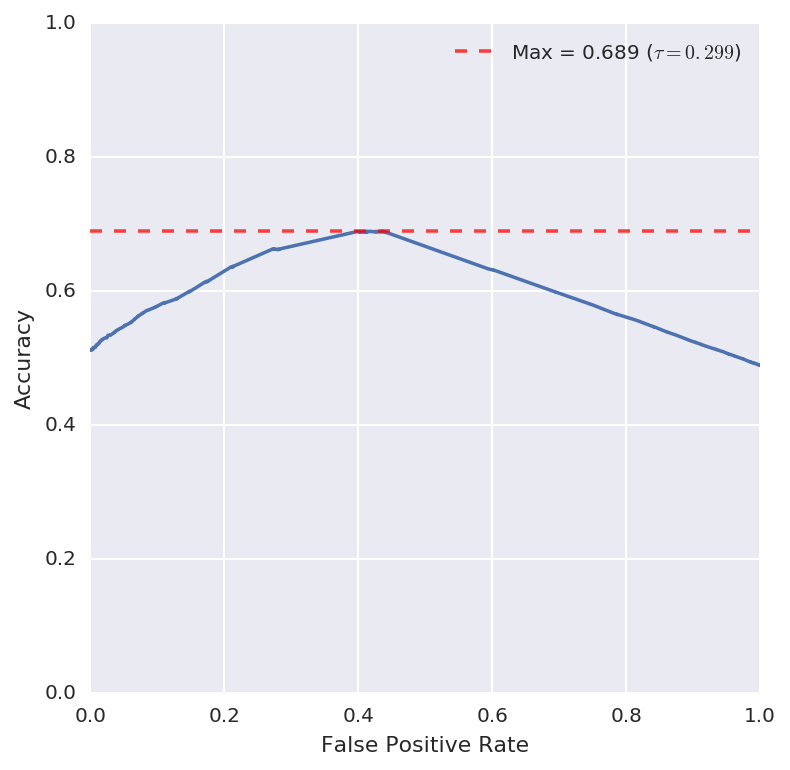
\includegraphics[width=\textwidth]{figures/bayes/accuracy_sms.png}
\end{subfigure}
\caption{Graphics representing the performance of the data when $\varpi = \sms$, using \emph{Beta Distributions} from the data in $\Upsilon^{\sms}$}
\end{figure}


\subsubsection{Inferring by Contacts}

\begin{figure}[h]
\centering
\begin{subfigure}[t]{\textwidth}
	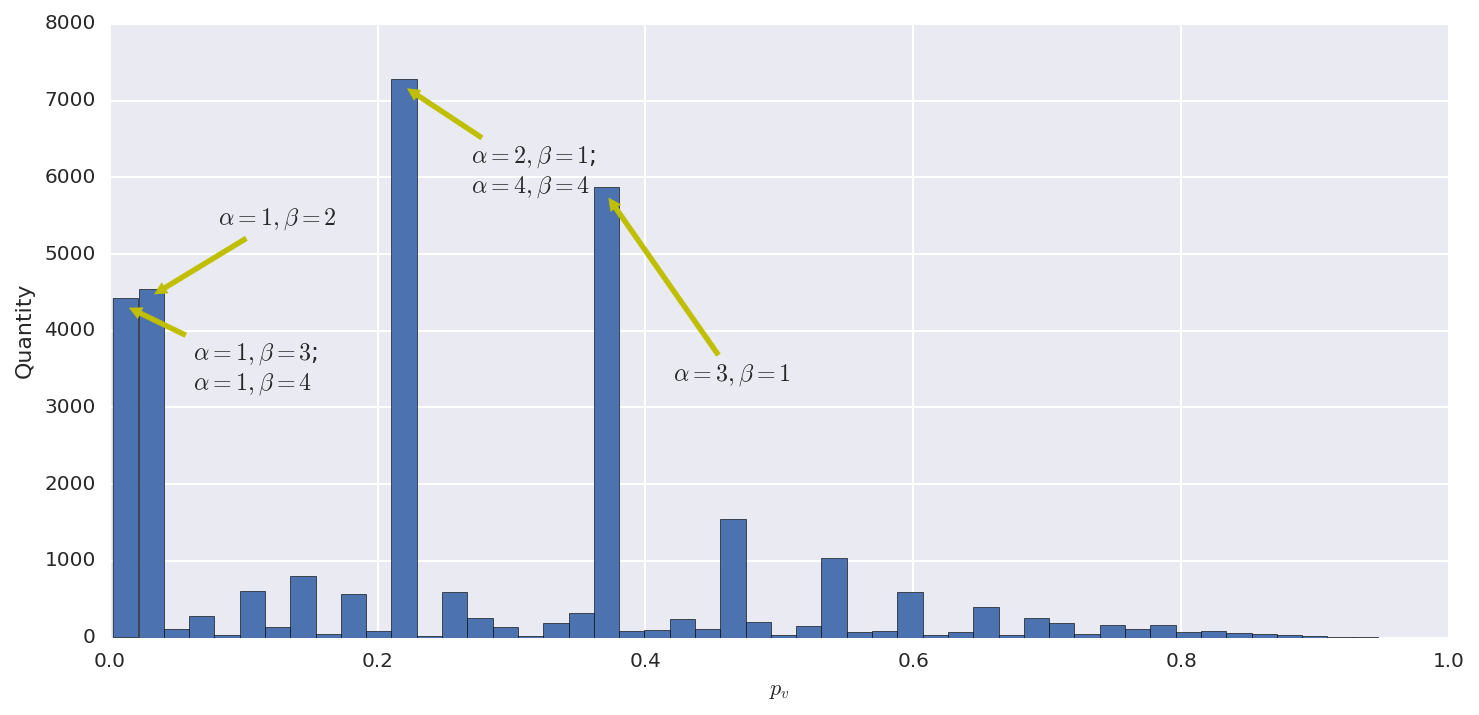
\includegraphics[width=\textwidth]{figures/bayes/hist_contacts.png}
\end{subfigure}

\begin{subfigure}[b]{.49\textwidth}
	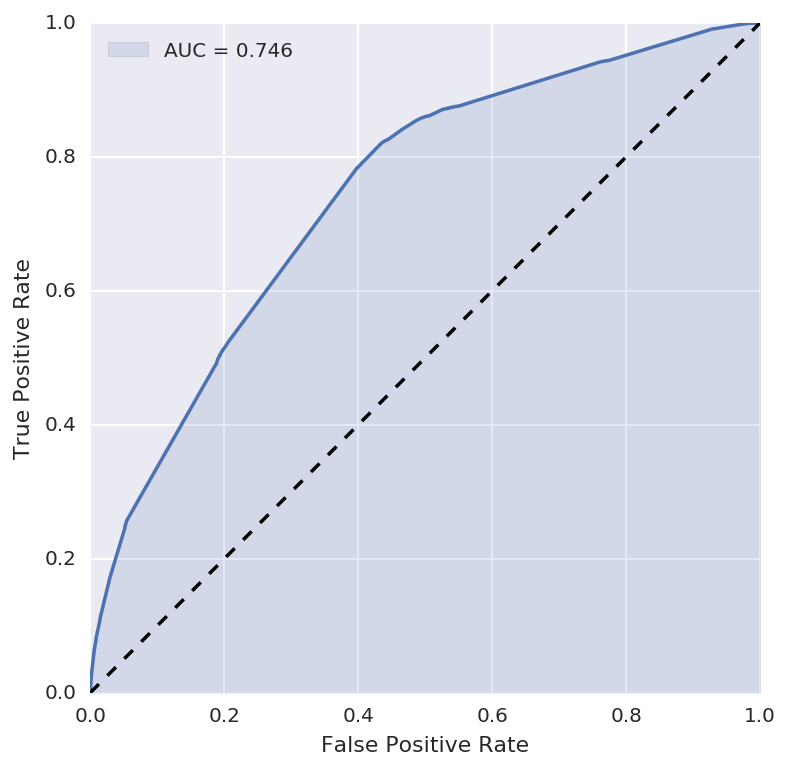
\includegraphics[width=\textwidth]{figures/bayes/roc_contacts.png}
\end{subfigure}
\begin{subfigure}[b]{.49\textwidth}
	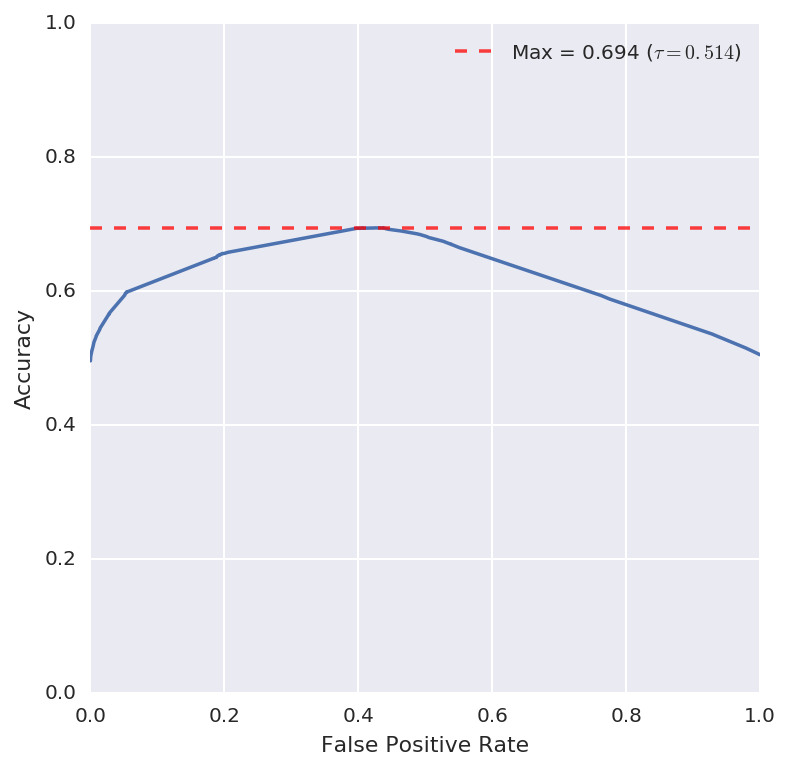
\includegraphics[width=\textwidth]{figures/bayes/accuracy_contacts.png}
\end{subfigure}
\caption{Graphics representing the performance of the data when $\varpi = \contacts$, using \emph{Beta Distributions} from the data in $\Upsilon$}
\end{figure}
